\documentclass[a4pape]{article}
\usepackage[utf8]{inputenc}
\usepackage{tikz}
\usepackage{pdflscape}
\usepackage{verbatim}
\usetikzlibrary{mindmap}
\usepackage[hidelinks,pdfencoding=auto]{hyperref}

% Information boxes
\newcommand*{\info}[4][16.3]{
  \node [ annotation, #3, scale=0.65, text width = #1em, inner sep = 2mm ] at (#2) {
  \list{$\bullet$}{\topsep=0pt\itemsep=0pt\parsep=0pt
    \parskip=0pt\labelwidth=8pt\leftmargin=8pt
    \itemindent=0pt\labelsep=2pt}
    #4
  \endlist
  };
}

%%%% Predefined Colors: black, blue, brown, cyan, darkgray, gray, green, lightgray, lime, magenta, olive, orange, pink, purple, red, teal, violet, white, yellow.

\pagestyle{empty}
\begin{document}

%%%%%%%%%%%%%%%%%%%%%%%%%%%%%%%%%%%%%%%% Überblick
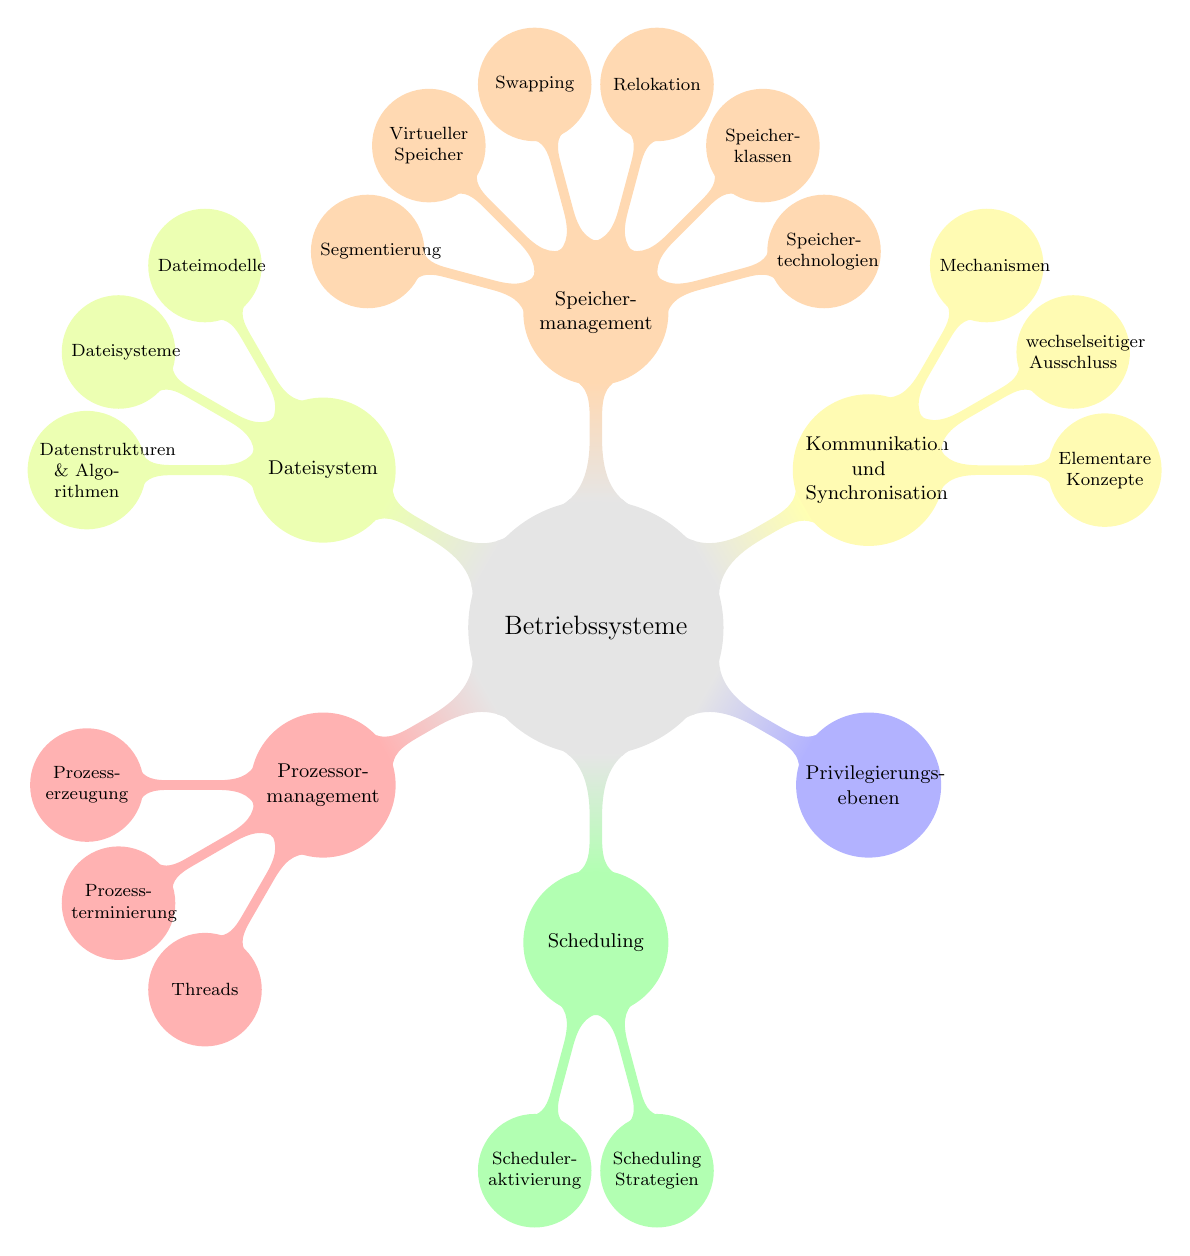
\begin{tikzpicture}[ mindmap, grow cyclic, every node/.style=concept, concept color=black!10,
    level 1/.append style={level distance=4cm},
    level 2/.append style={level distance=3cm, sibling angle=30},
    every node/.append style={scale=0.8}]

  \node{Betriebssysteme}
  child [concept color=red!30]{ node {Prozessor-management}
      child { node {Prozess-erzeugung}}
      child { node {Prozess-terminierung}}
      child { node {Threads}}
    }
  child [concept color=green!30]{ node {Scheduling}
      child { node {Scheduler-aktivierung}}
      child { node {Scheduling Strategien}}
    }
  child [concept color=blue!30]{ node {Privilegierungs-ebenen}}
  child [concept color=yellow!30]{ node {Kommunikation und\\Synchronisation}
      child { node {Elementare Konzepte}}
      child { node {wechselseitiger Ausschluss}}
      child { node {Mechanismen}}
    }
  child [concept color=orange!30]{ node {Speicher-management}
      child { node {Speicher-technologien}}
      child { node {Speicher-klassen}}
      child { node {Relokation}}
      child { node {Swapping}}
      child { node {Virtueller Speicher}}
      child { node {Segmentierung}}
    }
  child [concept color=lime!30]{ node {Dateisystem}
      child { node {Dateimodelle}}
      child { node {Dateisysteme}}
      child { node {Datenstrukturen \& Algorithmen}}
    };
\end{tikzpicture}

%%%%%%%%%%%%%%%%%%%%%%%%%%%%%%%%%%%%%% Grundbegriffe
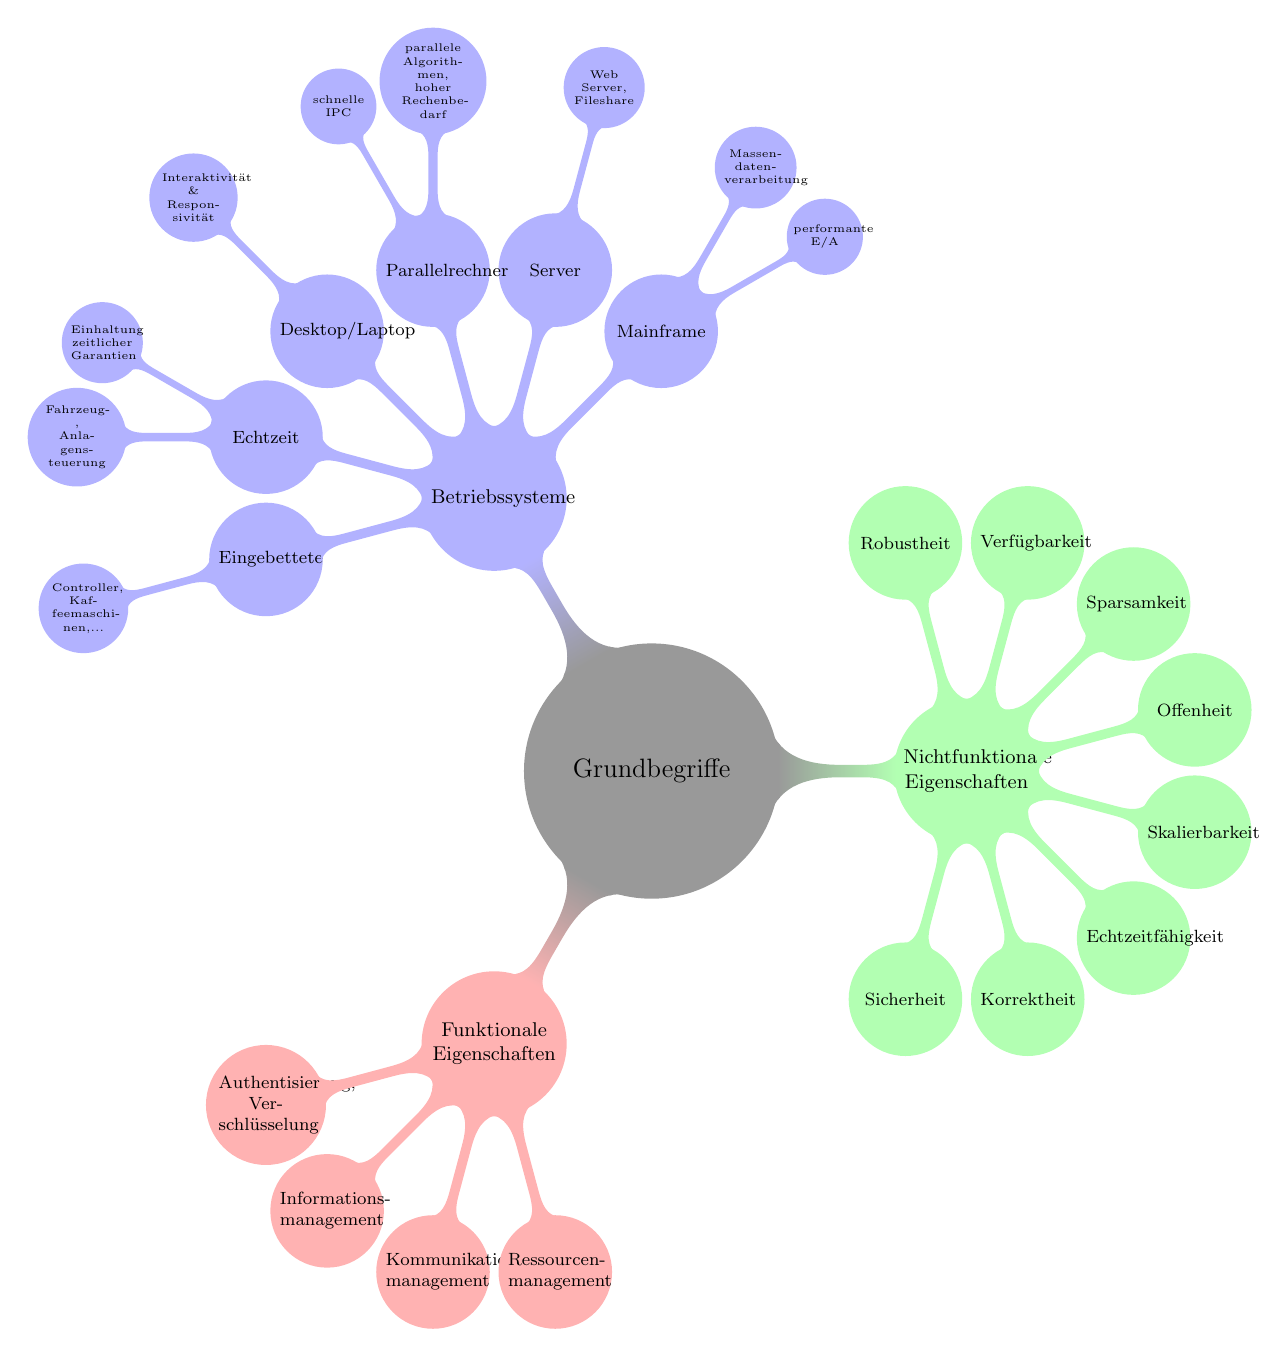
\begin{tikzpicture}[ mindmap, grow cyclic, every node/.style=concept, concept color=black!40,
    level 1/.append style={level distance=4cm, sibling angle=120},
    level 2/.append style={level distance=3cm, sibling angle=30},
    every node/.append style={scale=0.8}]
  \node{Grundbegriffe}
  child[concept color=red!30]{node{Funktionale Eigenschaften}
      child{node{Authentisierung, Verschlüsselung}}
      child{node{Informations-management}}
      child{node{Kommunikations-management}}
      child{node{Ressourcen-management}}
    }
  child[concept color=green!30]{node{Nichtfunktionale Eigenschaften}
      child{node{Sicherheit}}
      child{node{Korrektheit}}
      child{node{Echtzeitfähigkeit}}
      child{node{Skalierbarkeit}}
      child{node{Offenheit}}
      child{node{Sparsamkeit}}
      child{node{Verfügbarkeit}}
      child{node{Robustheit}}
    }
  child[concept color=blue!30]{node{Betriebssysteme}
      child{ node {Mainframe}
          child{ node {performante E/A}}
          child{ node {Massen-daten-verarbeitung}}
        }
      child{ node {Server}
          child{ node {Web Server, Fileshare}}
        }
      child{ node {Parallelrechner}
          child{ node {parallele Algorithmen, hoher Rechenbedarf}}
          child{ node {schnelle IPC}}
        }
      child{ node {Desktop/Laptop}
          child{ node {Interaktivität \& Responsivität}}
        }
      child{ node {Echtzeit}
          child{ node {Einhaltung zeitlicher Garantien}}
          child{ node {Fahrzeug-, Anlagensteuerung}}
        }
      child{ node {Eingebettete}
          child{ node {Controller, Kaffeemaschinen,...}}
        }
    }
  ;
\end{tikzpicture}

%%%%%%%%%%%%%%%%%%%%%%%%%%%%%%%%%%%%%% Prozessormanagement
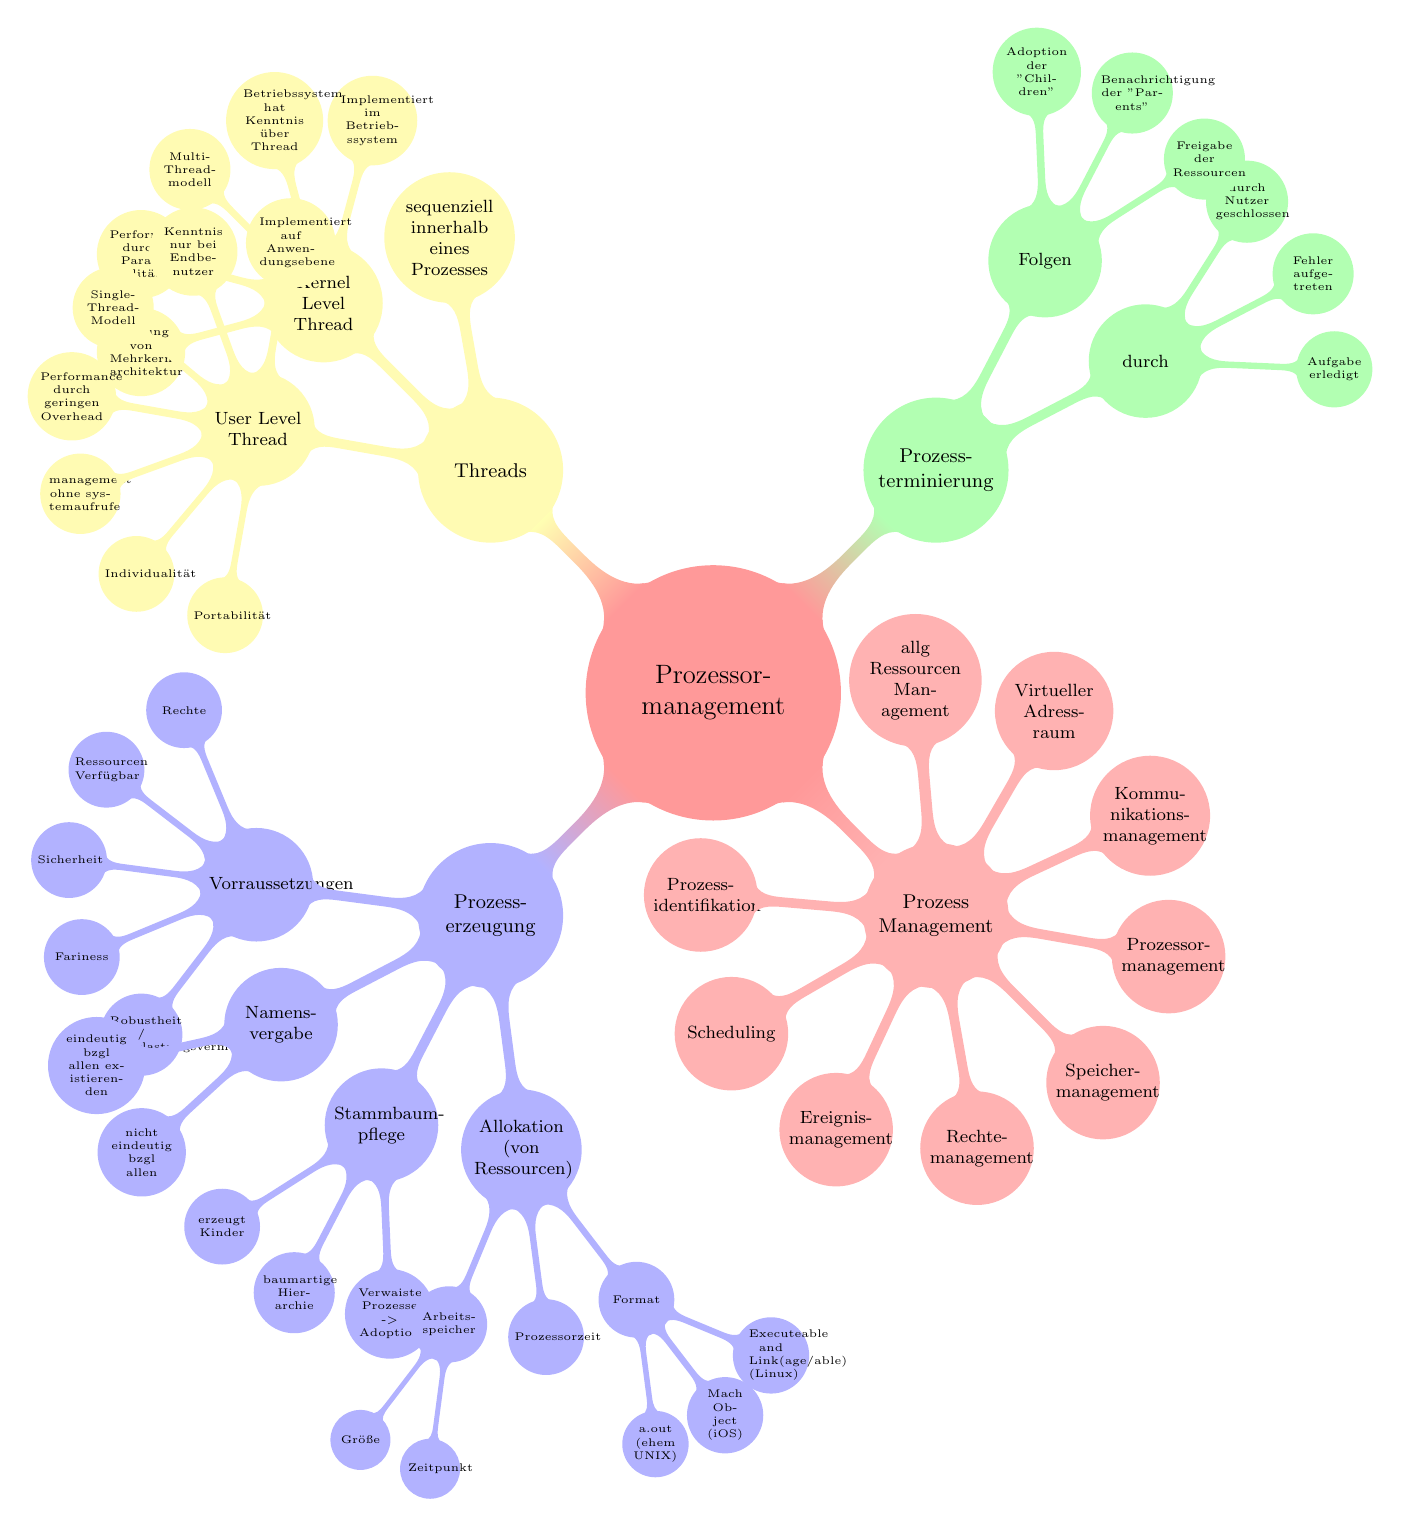
\begin{tikzpicture}[ mindmap, grow cyclic, every node/.style=concept, concept color=red!40,
    level 1/.append style={level distance=4cm, sibling angle=90},
    level 2/.append style={level distance=3cm, sibling angle=35},
    every node/.append style={scale=0.8}]
  \node{Prozessor-management}
  child[concept color=blue!30]  { node {Prozess-erzeugung}
      child { node {Vorraussetzungen}
          child { node {Rechte}}
          child{ node {Ressourcen Verfügbar}}
          child{ node {Sicherheit}}
          child{ node{Fariness}}
          child{node{Robustheit / Überlastungsvermeidung}}
        }
      child { node {Namens-vergabe}
          child{node{eindeutig bzgl allen existierenden}}
          child{node{nicht eindeutig bzgl allen}}
        }
      child { node {Stammbaum-pflege}
          child{node{erzeugt Kinder}}
          child{node{baumartige Hierarchie}}
          child{node{Verwaiste Prozesse -> Adoption}}
        }
      child { node {Allokation (von Ressourcen)}
          child{node{Arbeits-speicher}
              child{node{Größe}}
              child{node{Zeitpunkt}}
            }
          child{node{Prozessorzeit}}
          child{node{Format}
              child{node{a.out (ehem UNIX)}}
              child{node{Mach Object (iOS)}}
              child{node{Executeable and Link(age/able) (Linux)}}
            }
        }
    }
  child[concept color=red!30]  { node {Prozess Management}
      child{node{Prozess-identifikation}}
      child{node{Scheduling}}
      child{node{Ereignis-management}}
      child{node{Rechte-management}}
      child{node{Speicher-management}}
      child{node{Prozessor-management}}
      child{node{Kommu-nikations-management}}
      child{node{Virtueller Adressraum}}
      child{node{allg Ressourcen Management}}
    }
  child[concept color=green!30]  { node {Prozess-terminierung}
      child{node{durch}
          child{node{Aufgabe erledigt}}
          child{node{Fehler aufgetreten}}
          child{node{durch Nutzer geschlossen}}
        }
      child{node{Folgen}
          child{node{Freigabe der Ressourcen}}
          child{node{Benachrichtigung der "Parents"}}
          child{node{Adoption der "Children"}}
        }
    }
  child[concept color=yellow!30]  { node {Threads}
      child{node{sequenziell innerhalb eines Prozesses}}
      child{node{Kernel Level Thread}
          child{node{Implementiert im Betriebssystem}}
          child{node{Betriebssystem hat Kenntnis über Thread}}
          child{node{Multi-Thread-modell}}
          child{node{Performance durch Parallelität}}
          child{node{Nutzung von Mehrkern-architektur}}
        }
      child{node{User Level Thread}
          child{node{Implementiert auf Anwendungsebene}}
          child{node{Kenntnis nur bei Endbenutzer}}
          child{node{Single-Thread-Modell}}
          child{node{Performance durch geringen Overhead}}
          child{node{management ohne systemaufrufe}}
          child{node{Individualität}}
          child{node{Portabilität}}
        }
    }
  ;
\end{tikzpicture}

%%%%%%%%%%%%%%%%%%%%%%%%%%%%%%%%%%%%%% Scheduling
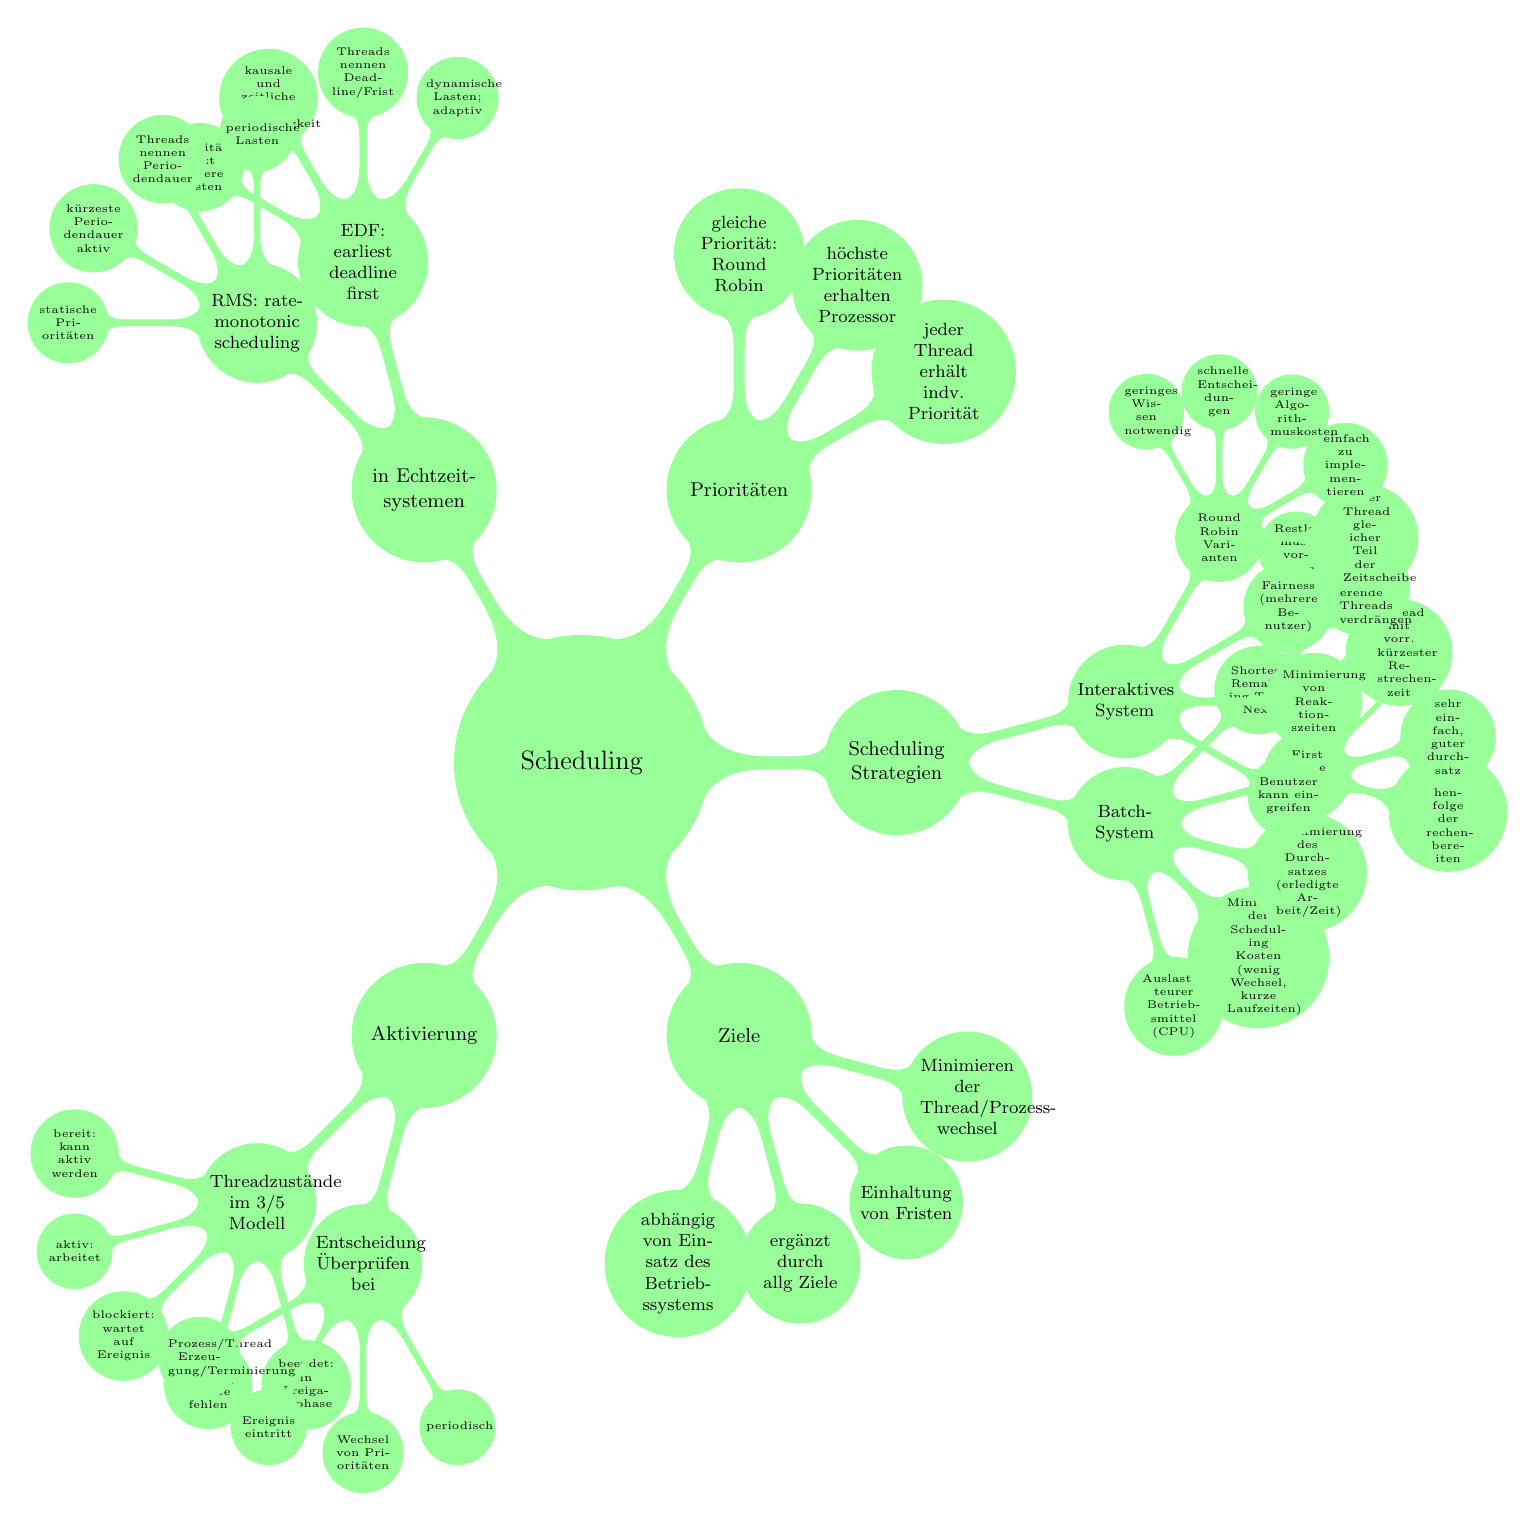
\begin{tikzpicture}[ mindmap, grow cyclic, every node/.style=concept, concept color=green!40,
    level 1/.append style={level distance=4cm},
    level 2/.append style={level distance=3cm, sibling angle=30},
    every node/.append style={scale=0.8}]
  \node{Scheduling}
  child { node {Aktivierung}
      child{node{Threadzustände im 3/5 Modell}
          child{node{bereit: kann aktiv werden}}
          child{node{aktiv: arbeitet}}
          child{node{blockiert: wartet auf Ereignis}}
          child{node{frisch: erzeugt, Rechte fehlen}}
          child{node{beendet: in Freigabephase}}
        }
      child{node{Entscheidung Überprüfen bei}
          child{node{Prozess/Thread Erzeugung/Terminierung}}
          child{node{Ereignis eintritt}}
          child{node{Wechsel von Prioritäten}}
          child{node{periodisch}}
        }
    }
  child{node{Ziele}
      child{node{abhängig von Einsatz des Betriebssystems}}
      child{node{ergänzt durch allg Ziele}}
      child{node{Einhaltung von Fristen}}
      child{node{Minimieren der Thread/Prozess-wechsel}}
    }
  child { node {Scheduling Strategien}
      child { node {Batch-System}
          child{node{Auslastung teurer Betriebsmittel (CPU)}}
          child{node{Minimierung der Scheduling Kosten (wenig Wechsel, kurze Laufzeiten)}}
          child{node{Maximierung des Durchsatzes (erledigte Arbeit/Zeit)}}
          child{node{First Come First Served}
              child{node{in Reihenfolge der rechenbereiten}}
              child{node{sehr einfach, guter durchsatz}}
              child{node{nicht immer klug}}
            }
          child{node{Shortest Remaining Time Next}
              child{node{Thread mit vorr. kürzester Restrechenzeit}}
              child{node{preemtiv; konkurrrierende Threads verdrängen}}
              child{node{Restlaufzeit muss vorliegen}}
            }
        }
      child { node {Interaktives System}
          child{node{Benutzer kann eingreifen}}
          child{node{Minimierung von Reaktionszeiten}}
          child{node{Fairness (mehrere Benutzer)}}
          child{node{Round Robin Varianten}
              child{node{jeder Thread gleicher Teil der Zeitscheibe}}
              child{node{einfach zu implementieren}}
              child{node{geringe Algorithmuskosten}}
              child{node{schnelle Entscheidungen}}
              child{node{geringes Wissen notwendig}}
            }
        }
    }
  child{node{Prioritäten}
      child{node{jeder Thread erhält indv. Priorität}}
      child{node{höchste Prioritäten erhalten Prozessor}}
      child{node{gleiche Priorität: Round Robin}}
    }
  child{node{in Echtzeitsystemen}
      child{node{EDF: earliest deadline first}
          child{node{dynamische Lasten; adaptiv}}
          child{node{Threads nennen Deadline/Frist}}
          child{node{kausale und zeitliche Unabhängigkeit}}
          child{node{Priorität setzt kürzere Fristen}}
        }
      child{node{RMS: rate-monotonic scheduling}
          child{node{periodische Lasten}}
          child{node{Threads nennen Periodendauer}}
          child{node{kürzeste Periodendauer aktiv}}
          child{node{statische Prioritäten}}
        }
    };
\end{tikzpicture}

%%%%%%%%%%%%%%%%%%%%%%%%%%%%%%%%%%%%%% Privilegierungsebenen
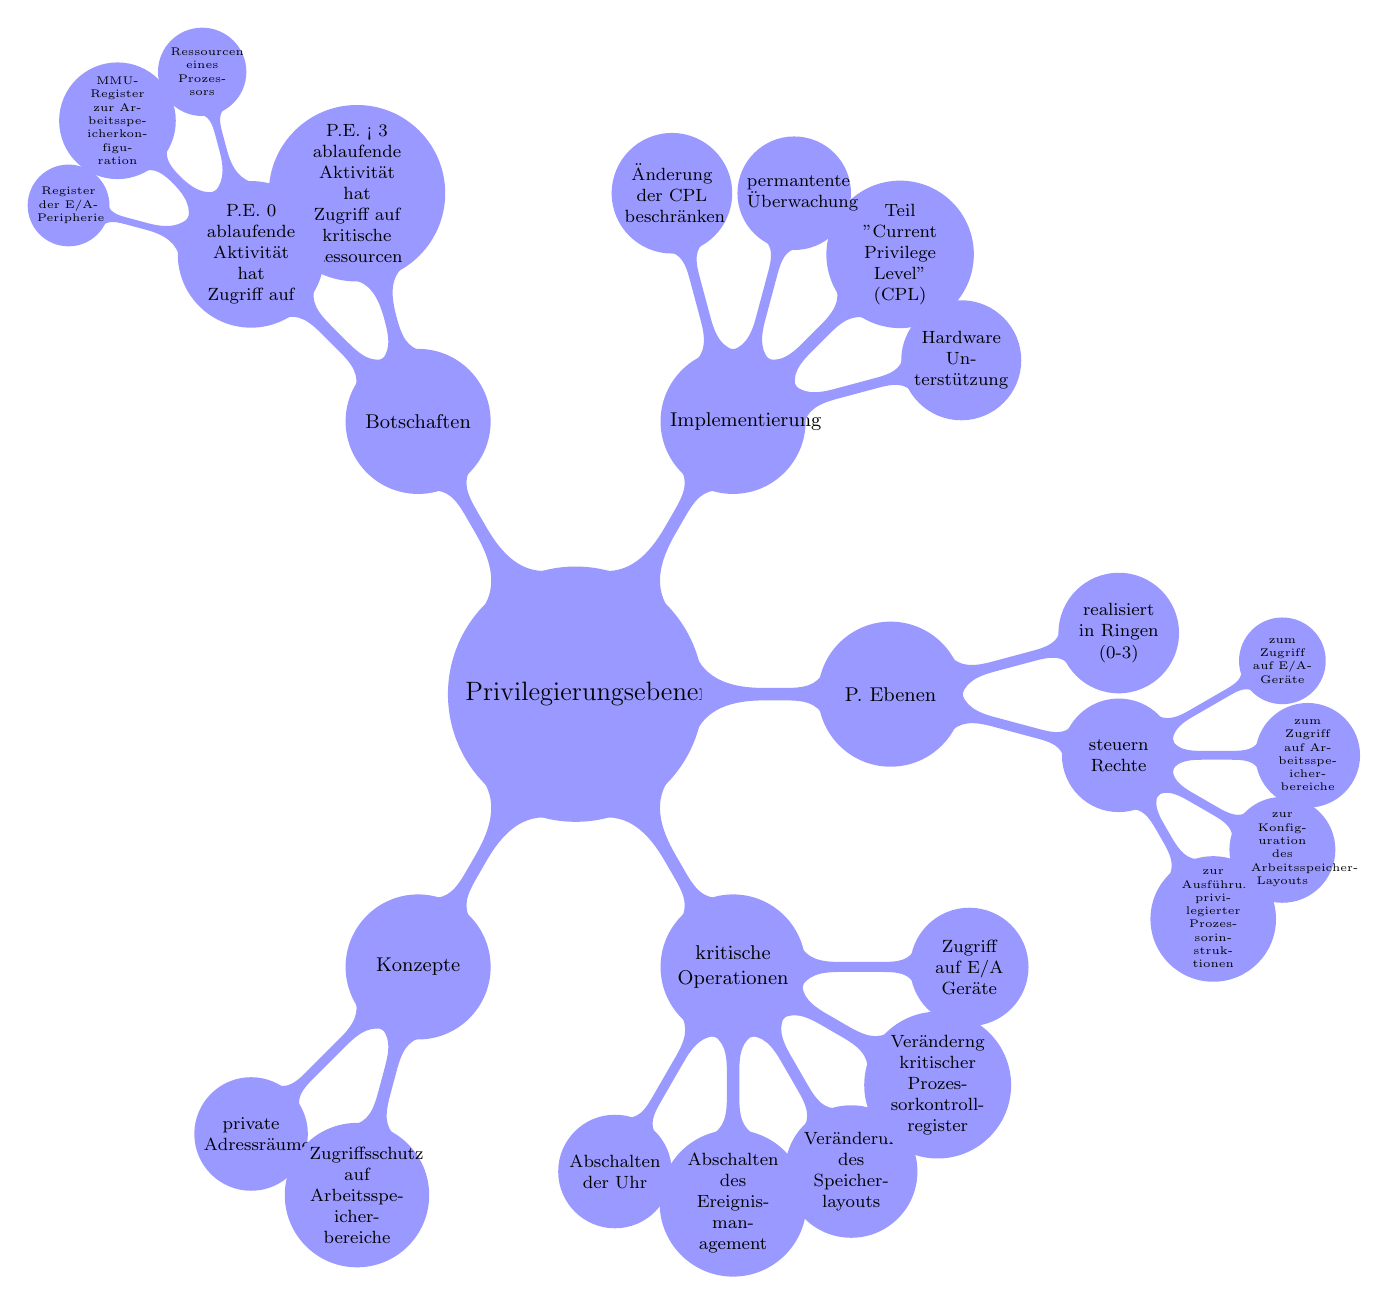
\begin{tikzpicture}[ mindmap, grow cyclic, every node/.style=concept, concept color=blue!40,
    level 1/.append style={level distance=4cm},
    level 2/.append style={level distance=3cm, sibling angle=30},
    every node/.append style={scale=0.8}]
  \node{Privilegierungsebenen}
  child{node{Konzepte}
      child{node{private Adressräume}}
      child{node{Zugriffsschutz auf Arbeitsspeicherbereiche}}
    }
  child{node{kritische Operationen}
      child{node{Abschalten der Uhr}}
      child{node{Abschalten des Ereignismanagement}}
      child{node{Veränderung des Speicherlayouts}}
      child{node{Veränderng kritischer Prozessorkontrollregister}}
      child{node{Zugriff auf E/A Geräte}}
    }
  child{node{P. Ebenen}
      child{node{steuern Rechte}
          child{node{zur Ausführung privilegierter Prozessorinstruktionen}}
          child{node{zur Konfiguration des Arbeitsspeicher-Layouts}}
          child{node{zum Zugriff auf Arbeitsspeicherbereiche}}
          child{node{zum Zugriff auf E/A-Geräte}}
        }
      child{node{realisiert in Ringen (0-3)}}
    }
  child{node{Implementierung}
      child{node{Hardware Unterstützung}}
      child{node{Teil "Current Privilege Level" (CPL)}}
      child{node{permantente Überwachung}}
      child{node{Änderung der CPL beschränken}}
    }
  child{node{Botschaften}
      child{node{P.E. < 3 ablaufende Aktivität hat Zugriff auf kritische Ressourcen}}
      child{node{P.E. 0 ablaufende Aktivität hat Zugriff auf}
          child{node{Ressourcen eines Prozessors}}
          child{node{MMU-Register zur Arbeitsspeicherkonfiguration}}
          child{node{Register der E/A-Peripherie}}
        }
    };
\end{tikzpicture}

%%%%%%%%%%%%%%%%%%%%%%%%%%%%%%%%%%%%%% Kommunikation und Synchronisation
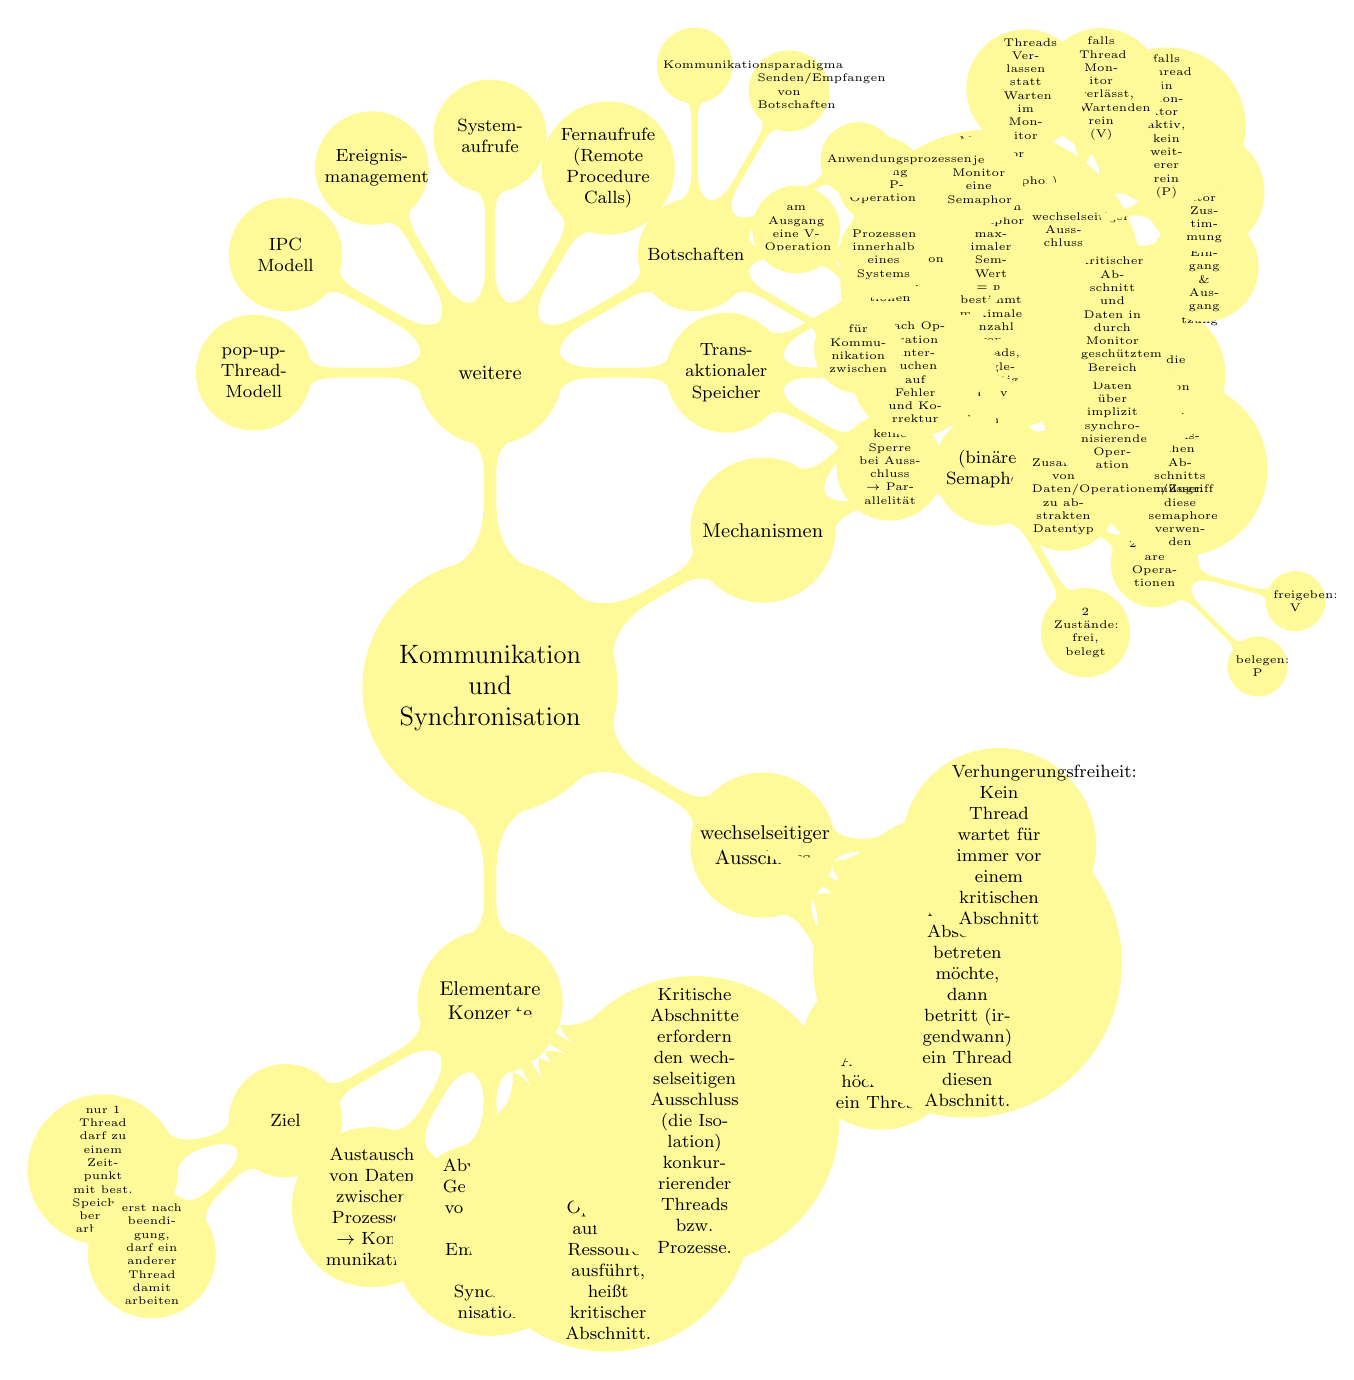
\begin{tikzpicture}[ mindmap, grow cyclic, every node/.style=concept, concept color=yellow!40,
    level 1/.append style={level distance=4cm},
    level 2/.append style={level distance=3cm, sibling angle=30},
    every node/.append style={scale=0.8}]
  \node{Kommunikation und \\Synchronisation}
  child { node {Elementare Konzepte}
      child{node{Ziel}
          child{node{nur 1 Thread darf zu einem Zeitpunkt mit best. Speicherbereich arbeiten}}
          child{node{erst nach beendigung, darf ein anderer Thread damit arbeiten}}
        }
      child{node{Austausch von Daten zwischen Prozessen $\rightarrow$ Kommunikation}}
      child{node{Abweichende Geschwindigkeiten von Sender und Empfänger $\rightarrow$ Synchronisation}}
      child{node{Eine Phase, in der ein Thread eine exklusive Operation auf einer Ressource ausführt, heißt kritischer Abschnitt.}}
      child{node{Kritische Abschnitte erfordern den wechselseitigen Ausschluss (die Isolation) konkurrierender Threads bzw. Prozesse.}}
    }
  child { node {wechselseitiger Ausschluss}
      child{node{Korrektheit: in kritischen Abschnitt höchstens ein Thread}}
      child{node{Lebendigkeit: Falls ein Thread einen kritischen Abschnitt betreten möchte, dann betritt (irgendwann) ein Thread diesen Abschnitt.}}
      child{node{Verhungerungsfreiheit: Kein Thread wartet für immer vor einem kritischen Abschnitt}}
    }
  child { node {Mechanismen}
      child { node {(binäre) Semaphore}
          child{node{2 Zustände: frei, belegt}}
          child{node{2 atomare Operationen}
              child{node{belegen: P}}
              child{node{freigeben: V}}
            }
          child{node{Sämtliche Nutzer dieses kritischen Abschnitts müssen diese semaphore verwenden}}
          child{node{Unterstützung durch Hardware: die TSL-Operation (TestAndSetLock)}}
          child{node{Implementierung im Ressourcenmanagement}}
          child{node{Mehrwertiger Semaphor (oder Zählsemaphor) mit mehreren Semaphoren; maximaler Sem-Wert = n, bestimmt maximale Anzahl von Threads, die gleichzeitig aktiv sein können}}
        }
      child { node {Hoare'sche Monitore}
          child{node{Zusammenfassen von Daten/Operationen/Zugriff zu abstrakten Datentyp}}
          child{node{Zugriff auf Daten über implizit synchronisierende Operation}}
          child{node{kritischer Abschnitt und Daten in durch Monitor geschütztem Bereich}}
          child{node{wechselseitiger Ausschluss}
              child{node{Türsteher an Eingang \& Ausgang}}
              child{node{Betreten nur mit Monitor Zustimmung}}
              child{node{falls Thread in Monitor aktiv, kein weiterer rein (P)}}
              child{node{falls Thread Monitor verlässt, Wartenden rein (V)}}
              child{node{Threads Verlassen statt Warten im Monitor}}
            }
          child{node{je Monitor eine Semaphor}}
          child{node{am Eingang eine P-Operation}}
          child{node{am Ausgang eine V-Operation}}
        }
    }
  child { node {weitere}
      child { node {Trans-aktionaler Speicher}
          child{node{keine Sperre bei Ausschluss $\rightarrow$ Parallelität}}
          child{node{nach Operation untersuchen auf Fehler und Korrektur}}
          child{node{Kombination mit Transaktionen}}
        }
      child { node {Botschaften}
          child{node{für Kommunikation zwischen}}
          child{node{Prozessen innerhalb eines Systems}}
          child{node{Anwendungsprozessen}}
          child{node{Senden/Empfangen von Botschaften}}
          child{node{Kommunikationsparadigma}}
        }
      child { node {Fernaufrufe (Remote Procedure Calls)}}
      child { node {System-aufrufe}}
      child { node {Ereignis-management}}
      child { node {IPC Modell}}
      child { node {pop-up-Thread-Modell}}
    };
\end{tikzpicture}

%%%%%%%%%%%%%%%%%%%%%%%%%%%%%%%%%%%%%% Speichermanagement
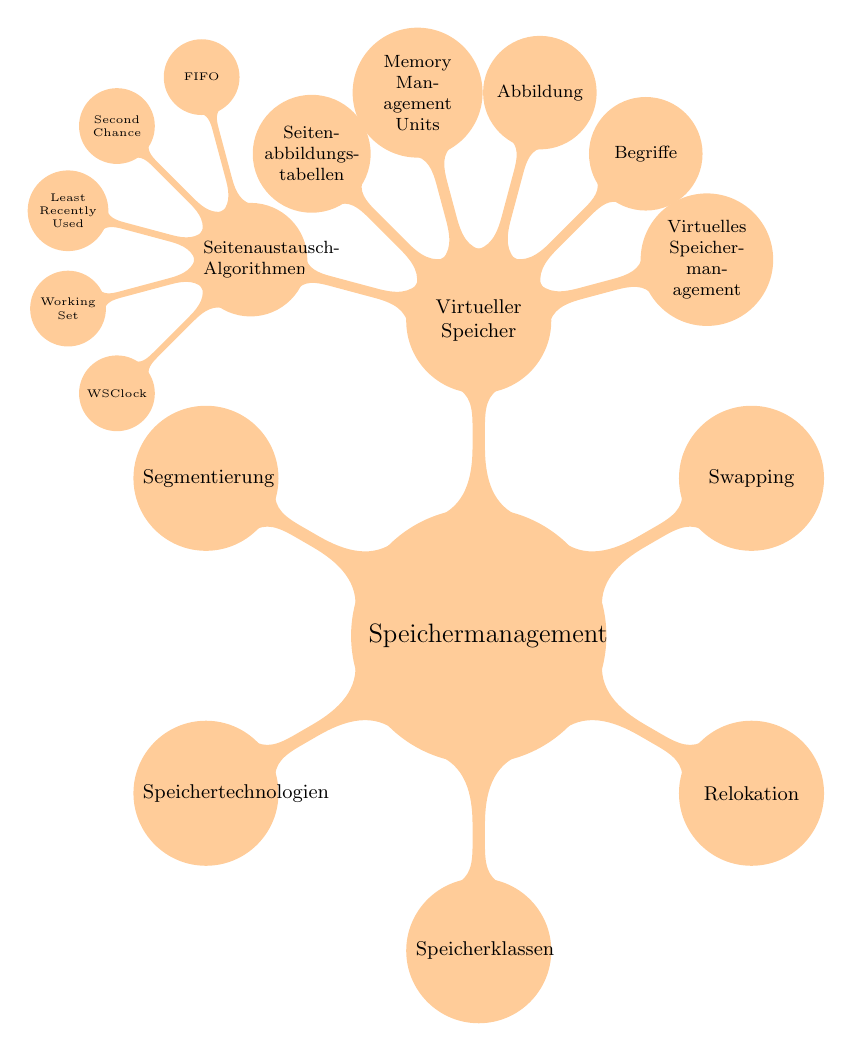
\begin{tikzpicture}[ mindmap, grow cyclic, every node/.style=concept, concept color=orange!40,
    level 1/.append style={level distance=4cm},
    level 2/.append style={level distance=3cm, sibling angle=30},
    every node/.append style={scale=0.8}]
  \node{Speichermanagement}
  child { node {Speichertechnologien }}
  child { node {Speicherklassen}}
  child { node {Relokation}}
  child { node {Swapping}}
  child { node {Virtueller Speicher}
      child { node {Virtuelles Speichermanagement}}
      child { node {Begriffe}}
      child { node {Abbildung}}
      child { node {Memory Management Units}}
      child { node {Seiten-abbildungs-tabellen}}
      child { node {Seitenaustausch-Algorithmen}
          child { node {FIFO}}
          child { node {Second Chance}}
          child { node {Least Recently Used}}
          child { node {Working Set}}
          child { node {WSClock}}
        }
    }
  child { node {Segmentierung}}
  ;
\end{tikzpicture}

%%%%%%%%%%%%%%%%%%%%%%%%%%%%%%%%%%%%%% Dateisystem
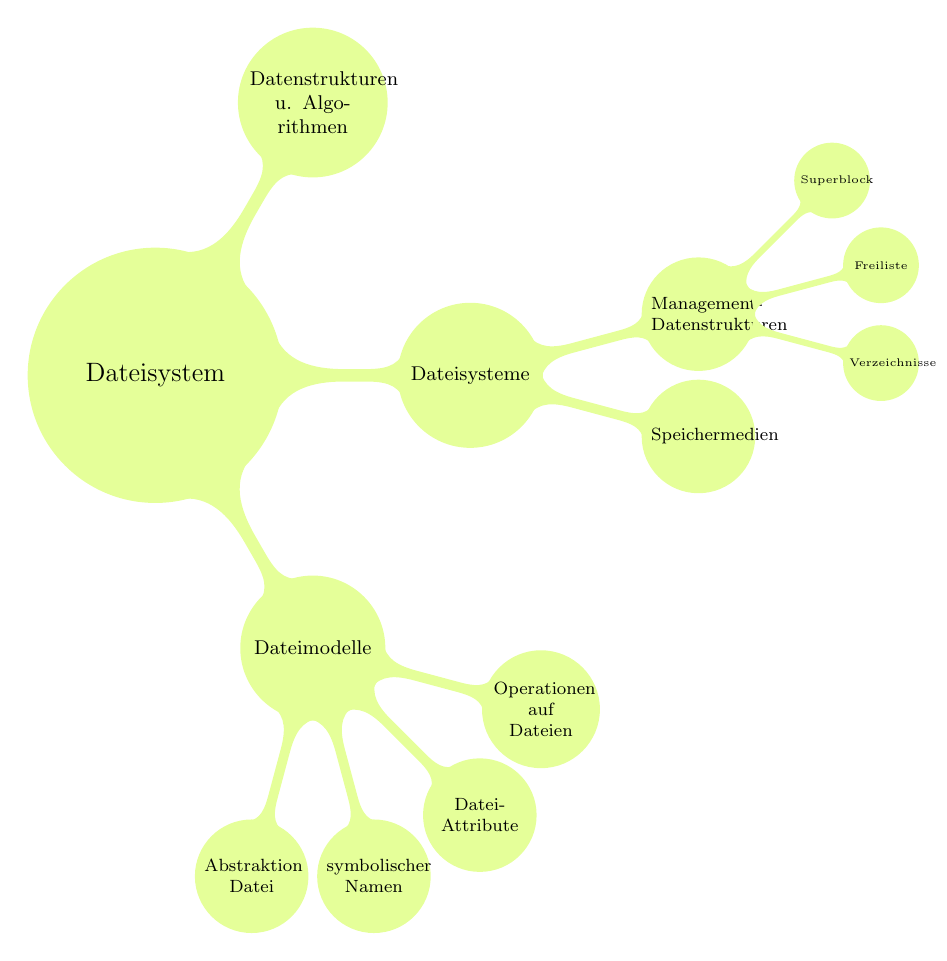
\begin{tikzpicture}[ mindmap, grow cyclic, every node/.style=concept, concept color=lime!40,
    level 1/.append style={level distance=4cm},
    level 2/.append style={level distance=3cm, sibling angle=30},
    every node/.append style={scale=0.8}]
  \node{Dateisystem}
  child { node {Dateimodelle}
      child { node {Abstraktion Datei}}
      child { node {symbolischer Namen}}
      child { node {Datei-Attribute}}
      child { node {Operationen auf Dateien}}
    }
  child { node {Dateisysteme}
      child { node {Speichermedien}}
      child { node {Management-Datenstrukturen}
          child { node {Verzeichnisse}}
          child { node {Freiliste}}
          child { node {Superblock}}
        }
    }
  child { node {Datenstrukturen u. Algorithmen}}
  ;
\end{tikzpicture}


\end{document}